% *********************************************************************
% © 2010–2026 Jeremy Sylvestre
%
% Permission is granted to copy, distribute and/or modify this document
% under the terms of the GNU Free Documentation License, Version 1.3 or
% any later version published by the Free Software Foundation; with no
% Invariant Sections, no Front-Cover Texts, and no Back-Cover Texts. A
% copy of the license is included in the appendix entitled “GNU Free
% Documentation License” that appears in the output document of this
% PreTeXt source code. All trademarks™ are the registered® marks of
% their respective owners.
%
% *********************************************************************

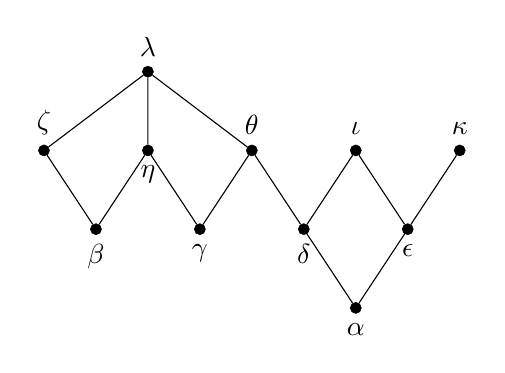
\begin{tikzpicture}[
	xscale=0.66,
	vertex/.style={ circle, draw, very thin, fill, inner sep=0pt, minimum size=4pt },
	vertexg/.style={ black!40!white, circle, draw, very thin, fill, inner sep=0pt, minimum size=4pt },
	vertexo/.style={ circle, draw, very thin, inner sep=0pt, minimum size=4pt }
]

\node at (2,0) (zero) [vertex,label=below:{$\alpha$}] {};
\node at (-3,1) (one) [vertex,label=below:{$\beta$}] {};
\node at (-1,1) (two) [vertex,label=below:{$\gamma$}] {};
\node at (1,1) (three) [vertex,label=below:{$\delta$}] {};
\node at (3,1) (four) [vertex,label=below:{$\epsilon$}] {};
\foreach \p in {three,four} \draw (zero) to (\p);

\node at (-4,2) (five) [vertex,label=above:{$\zeta$}] {};
\node at (-2,2) (six) [vertex,label=below:{$\eta$}] {};
\node at (0,2) (seven) [vertex,label=above:{$\theta$}] {};
\node at (2,2) (eight) [vertex,label=above:{$\iota$}] {};
\node at (4,2) (nine) [vertex,label=above:{$\kappa$}] {};
\foreach \p in {five,six} \draw (one) to (\p);
\foreach \p in {six,seven} \draw (two) to (\p);
\foreach \p in {seven,eight} \draw (three) to (\p);
\foreach \p in {eight,nine} \draw (four) to (\p);

\node at (-2,3) (ten) [vertex,label=above:{$\lambda$}] {};
\foreach \p in {five,six,seven} \draw (\p) to (ten);


% \foreach \p in {four,five} \draw (\p) to (seven);

\end{tikzpicture}
